\documentclass[aspectratio=169]{beamer}
\usetheme{metropolis}

\usepackage[spanish]{babel}
\usepackage[utf8]{inputenc}
\usepackage{graphicx}
\usepackage{tikz}
\usepackage{xcolor}
\usepackage{amsmath}
\usepackage{booktabs}

\definecolor{primary}{RGB}{46, 204, 113}
\definecolor{accent}{RGB}{231, 76, 60}
\definecolor{background}{RGB}{236, 240, 241}
\setbeamercolor{normal text}{fg=black,bg=background}
\setbeamercolor{structure}{fg=primary}
\setbeamercolor{alerted text}{fg=accent}

\newcommand{\udesalogo}[1]{%
\begin{tikzpicture}[remember picture,overlay]
    \node[anchor=#1,inner sep=30pt] at (current page.#1) {
\includegraphics[height=1cm]{../misc/UdeSA.png}};
\end{tikzpicture}}

\title{\Huge\textbf{Aprendizaje No Supervisado}}
\subtitle{K-means, clustering jerárquico y PCA}
\author{Analítica de Datos, Universidad de San Andrés}
\date{}

\begin{document}

\begin{frame}
    \titlepage
    \udesalogo{south west}
\end{frame}

% =====================================================================
\begin{frame}{Hasta ahora: aprendizaje supervisado}
    \begin{columns}[T]
        \column{0.48\textwidth}
        \textbf{Supervisado} (CART, KNN, RF, Naive Bayes)
        \begin{itemize}
            \item Tenemos una columna \alert{respuesta}: ¿pagó?, ¿compró?, ¿precio?
            \item El modelo aprende a \textbf{predecirla}
            \item Podemos medir si acierta (accuracy, ROC, ...)
        \end{itemize}
        \column{0.48\textwidth}
        \textbf{No supervisado} (hoy)
        \begin{itemize}
            \item \alert{No hay respuesta}: solo tenemos las características
            \item Buscamos \textbf{estructura}: grupos, patrones, resúmenes
            \item No hay ``acierto'': la utilidad la decide el negocio
        \end{itemize}
    \end{columns}
    \vspace{1em}
    \begin{center}
        \textit{``No sé qué tipos de clientes tengo''} vs. \textit{``Sé quién se fue, quiero predecir quién se va a ir''}
    \end{center}
\end{frame}

\begin{frame}{Tres preguntas de negocio, tres técnicas}
    \centering
    \renewcommand{\arraystretch}{1.5}
    \begin{tabular}{p{5.4cm}p{3.3cm}p{4.6cm}}
        \toprule
        \textbf{Pregunta} & \textbf{Técnica} & \textbf{Demo de hoy} \\
        \midrule
        ¿Qué tipos de clientes tengo? ¿A quién le mando qué campaña? & \textbf{K-means} & 200 clientes de un shopping \\
        ¿Qué países se parecen entre sí para expandirme? & \textbf{Clustering jerárquico} & 193 países (ONU) \\
        Tengo 12 métricas que dicen lo mismo: ¿cómo las resumo en un mapa? & \textbf{PCA} & 93 modelos de autos \\
        \bottomrule
    \end{tabular}
    \vspace{0.8em}

    Las dos primeras \textbf{agrupan filas} (clientes, países). PCA \textbf{resume columnas} (variables).
\end{frame}

% =====================================================================
\section{K-means: segmentar clientes}

\begin{frame}{El problema}
    \begin{columns}[c]
        \column{0.55\textwidth}
        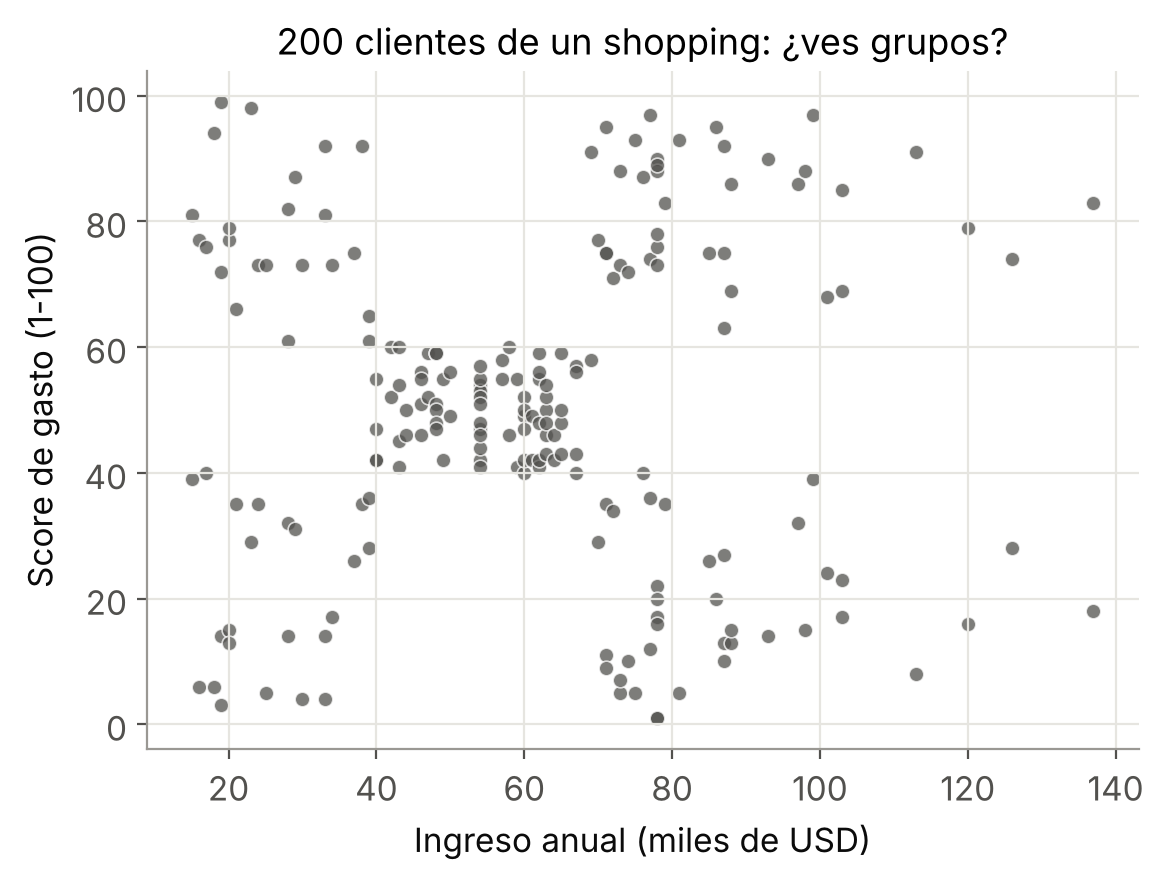
\includegraphics[width=\textwidth]{img/km_datos.png}
        \column{0.42\textwidth}
        Marketing de un shopping. Por cada cliente de la tarjeta de fidelidad tenemos:
        \begin{itemize}
            \item Ingreso anual
            \item Score de gasto (1--100)
        \end{itemize}
        \vspace{0.5em}
        Queremos armar campañas para \alert{distintos tipos de clientes}, pero nadie nos dijo cuáles son.
        \vspace{0.5em}

        \textbf{¿Cuántos grupos ves?}
    \end{columns}
\end{frame}

\begin{frame}{La idea: K ``clientes representantes''}
    \centering
    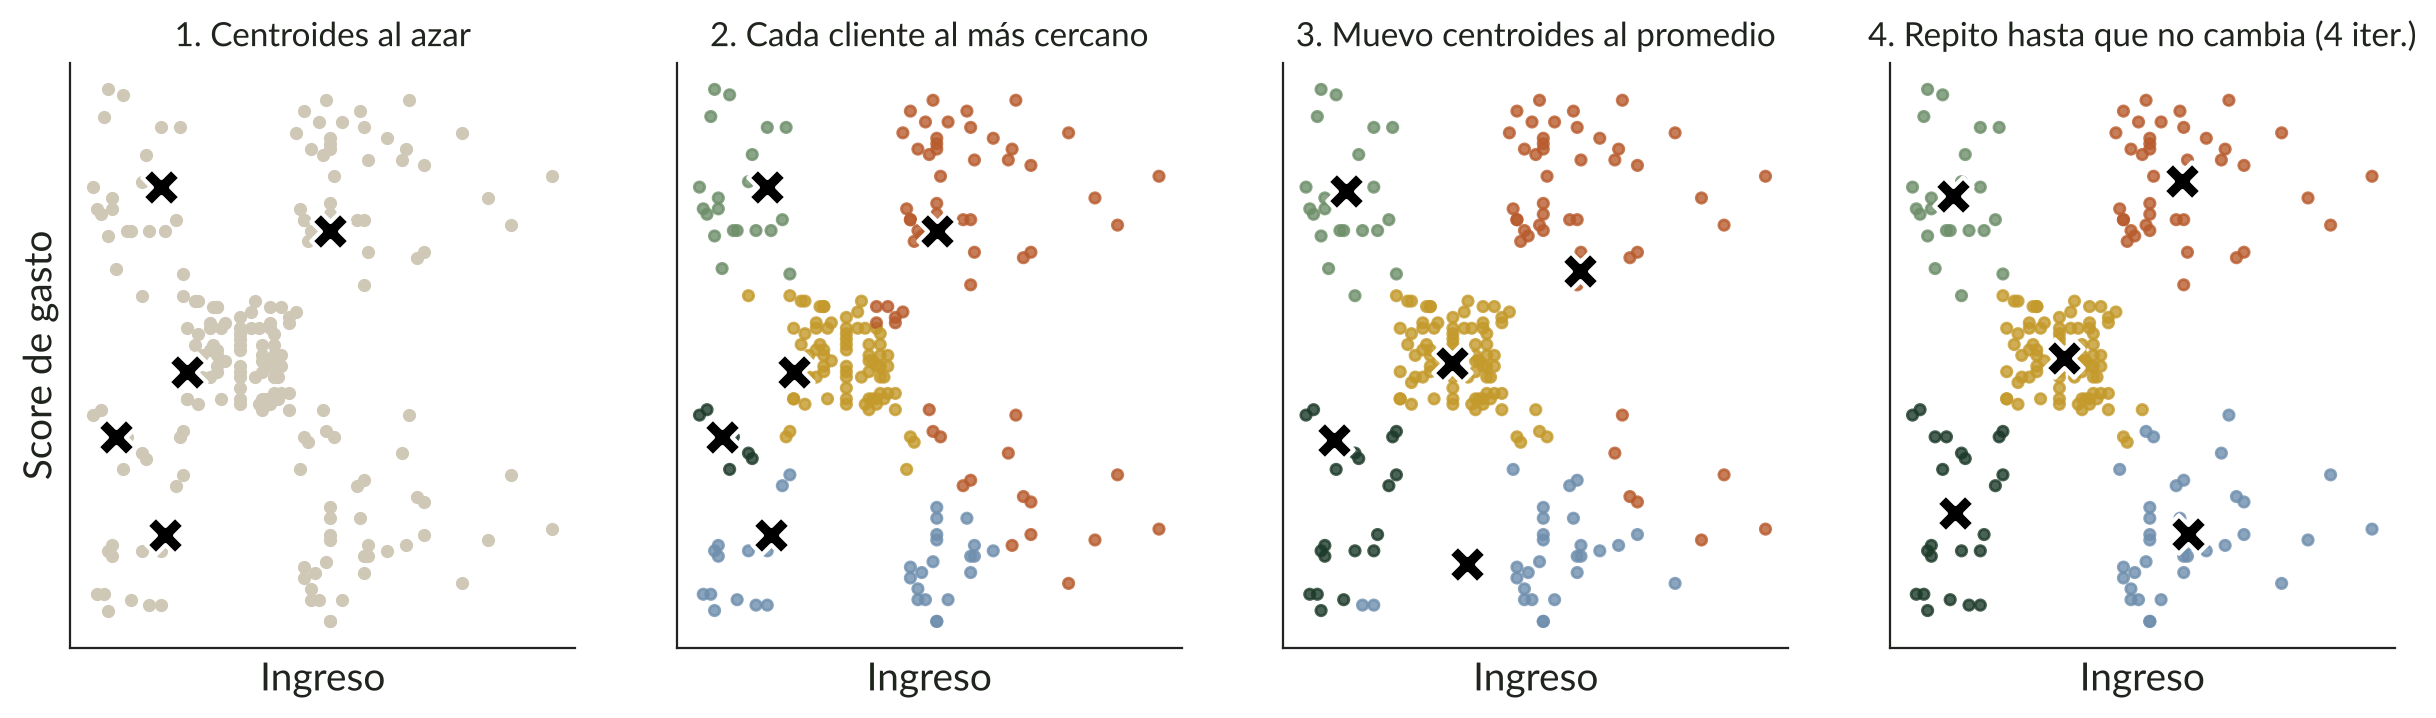
\includegraphics[width=\textwidth]{img/km_pasos.png}
    \vspace{0.3em}

    \small Elegimos \textbf{K} y tiramos K centroides al azar. Cada cliente se asigna al centroide más cercano, cada centroide se mueve al promedio de sus clientes, y repetimos hasta que nada cambia.
\end{frame}

\begin{frame}{La matemática, muy por arriba}
    K-means busca los grupos que minimizan la \alert{inercia}:
    \[
        \text{Inercia} = \sum_{\text{grupos}} \; \sum_{\text{clientes del grupo}} \text{distancia}(\text{cliente}, \text{centroide})^2
    \]
    \begin{itemize}
        \item Traducción: \textbf{grupos lo más ``apretados'' posible} alrededor de su representante.
        \item ``Distancia'' = distancia en línea recta (euclídea) entre los valores de las variables.
        \item Por eso hay que \alert{estandarizar}: si el ingreso está en pesos y el score en 1--100, el ingreso domina la distancia.
        \item El resultado depende del arranque al azar $\Rightarrow$ se corre varias veces y se queda con la mejor (\texttt{n\_init=10}).
    \end{itemize}
\end{frame}

\begin{frame}{¿Cuántos grupos? K lo elegimos nosotros}
    \centering
    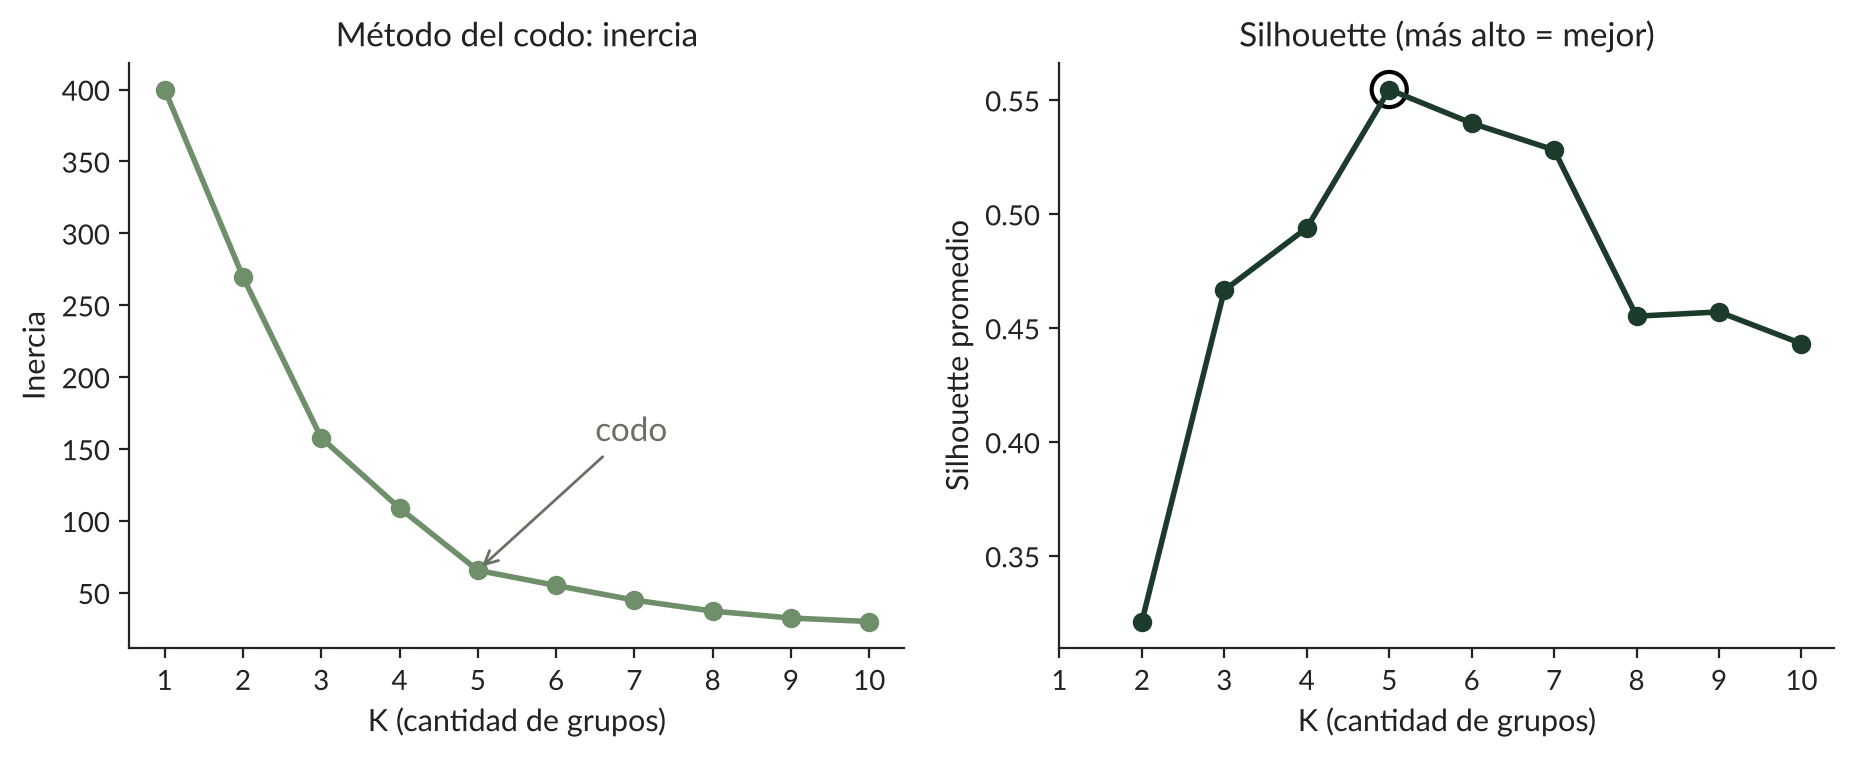
\includegraphics[width=0.85\textwidth]{img/km_elegir_k.png}
    \begin{itemize}\small
        \item \textbf{Codo}: la inercia siempre baja al agregar grupos; buscamos donde \textit{deja de bajar mucho}.
        \item \textbf{Silhouette}: ¿cada cliente está más cerca de su grupo que del grupo vecino? (de $-1$ a $1$).
        \item Y una pregunta de negocio: \alert{¿cuántas campañas distintas puede manejar el equipo?}
    \end{itemize}
\end{frame}

\begin{frame}{El algoritmo da números; el nombre lo ponemos nosotros}
    \begin{columns}[c]
        \column{0.58\textwidth}
        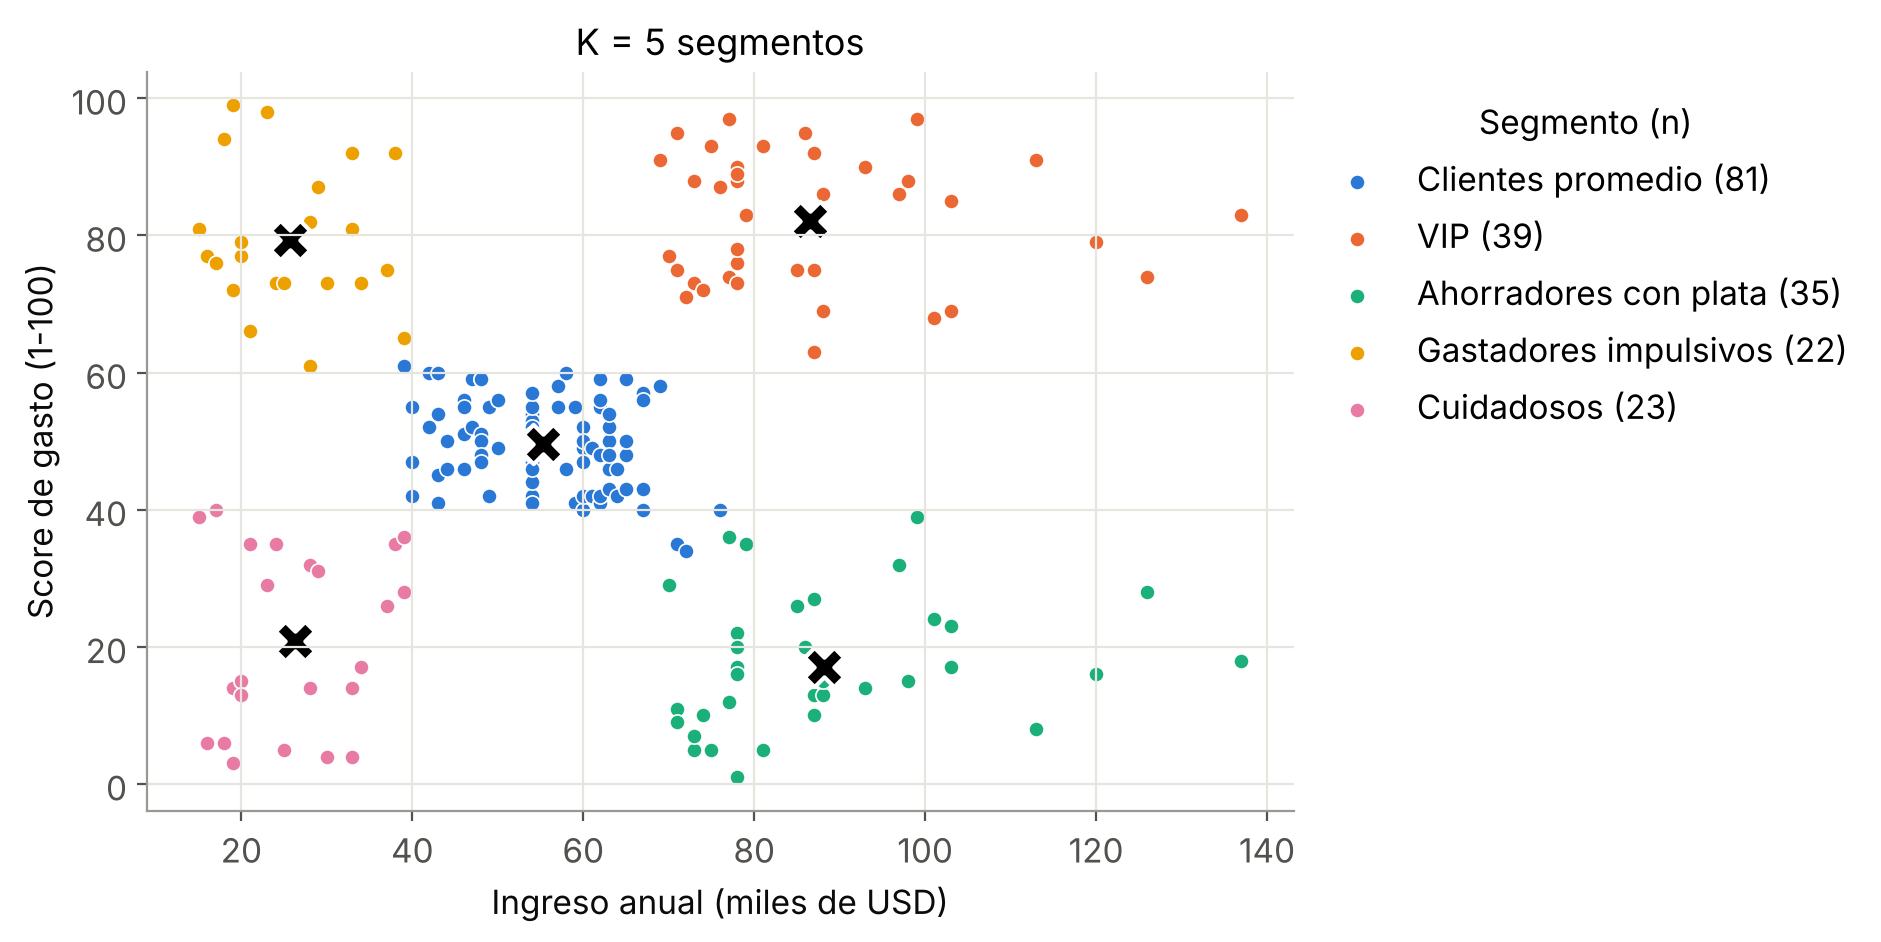
\includegraphics[width=\textwidth]{img/km_segmentos.png}
        \column{0.40\textwidth}
        \footnotesize
        \begin{tabular}{@{}p{2.3cm}p{3.3cm}@{}}
            \toprule
            \textbf{Segmento} & \textbf{Acción} \\
            \midrule
            VIP & Fidelizar, eventos exclusivos \\
            Ahorradores con plata & \alert{Mayor potencial}: ¿por qué no compran acá? \\
            Gastadores impulsivos & Promos, cuotas; son los más jóvenes \\
            Cuidadosos & Descuentos puntuales \\
            Promedio & Comunicación masiva \\
            \bottomrule
        \end{tabular}
    \end{columns}
\end{frame}

\begin{frame}{Cuidado con K-means}
    \begin{itemize}
        \item \textbf{Siempre devuelve K grupos}, aunque los datos no tengan grupos.
        \item \textbf{Estandarizar} las variables antes (trabaja con distancias).
        \item Le gustan los grupos \textbf{redondos y de tamaño parecido}; con formas raras falla.
        \item \textbf{Outliers} tiran de los centroides.
        \item Solo variables \textbf{numéricas} (las categóricas hay que codificarlas con cuidado).
        \item Escala muy bien: funciona con millones de clientes.
    \end{itemize}
\end{frame}

\begin{frame}[standout]
    \centering
    {\Large Demo 1: segmentación de clientes\par}
    \vspace{0.6em}
    {\normalsize\texttt{01\_kmeans\_clientes.ipynb}\par}
\end{frame}

% =====================================================================
\section{Clustering jerárquico: agrupar países}

\begin{frame}{El problema}
    Una \textbf{fintech argentina} quiere expandirse. Antes de estudiar mercado por mercado:
    \begin{center}
        \Large \textit{¿Qué países se parecen entre sí?}
    \end{center}
    \begin{itemize}
        \item 193 países, 5 indicadores de la ONU: fertilidad, PBI per cápita, esperanza de vida, \% urbano, mortalidad infantil.
        \item \alert{No sabemos cuántos grupos hay} y queremos algo fácil de mostrarle al directorio.
        \item Si una estrategia funciona en un país, probablemente funcione en sus ``vecinos''.
    \end{itemize}
\end{frame}

\begin{frame}{La idea en una frase}
    \begin{center}
        \Large Arranco con cada país solo y \alert{voy juntando de a dos} \\ a los más parecidos, hasta que queda un solo grupo.
    \end{center}
    \vspace{1em}
    \begin{itemize}
        \item Es como armar un \textbf{árbol genealógico} de parecidos: primero se juntan los ``hermanos'', después los ``primos'', y así.
        \item El \textbf{dendrograma} es el dibujo de ese árbol: anota \textbf{quién} se juntó con quién y \textbf{qué tan distintos} eran cuando se juntaron.
        \item No hace falta elegir K antes: la cantidad de grupos se decide \textbf{al final}, mirando el árbol.
    \end{itemize}
    \vspace{0.5em}
    Veámoslo con 7 puntos, paso por paso $\rightarrow$
\end{frame}

\begin{frame}{Paso a paso: cómo se arma el árbol}
    \centering
    \only<1>{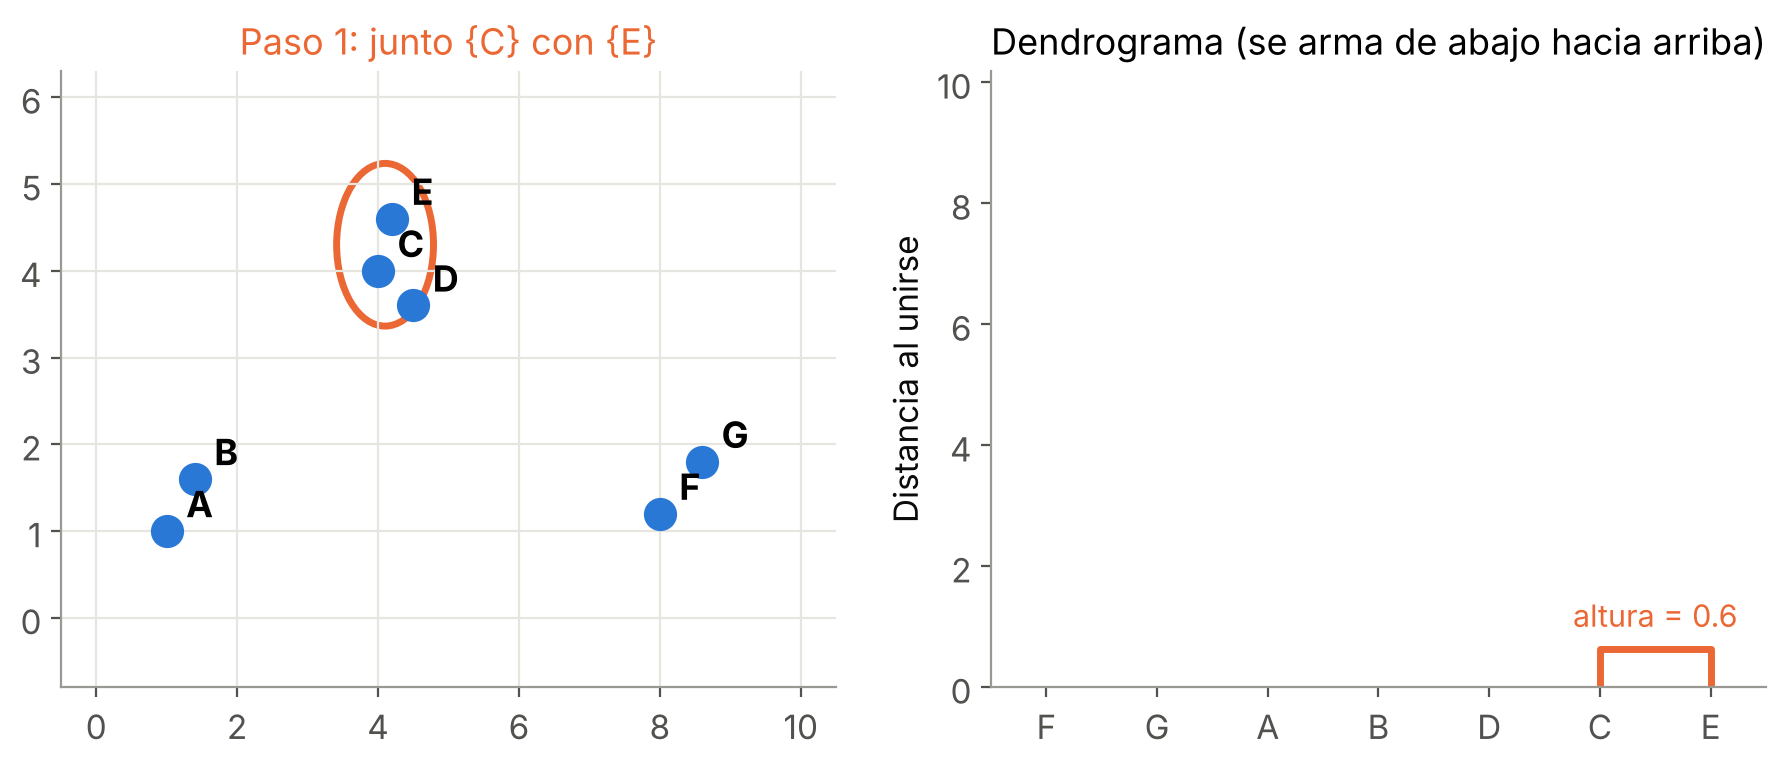
\includegraphics[width=0.88\textwidth]{img/jer_paso1.png}}%
    \only<2>{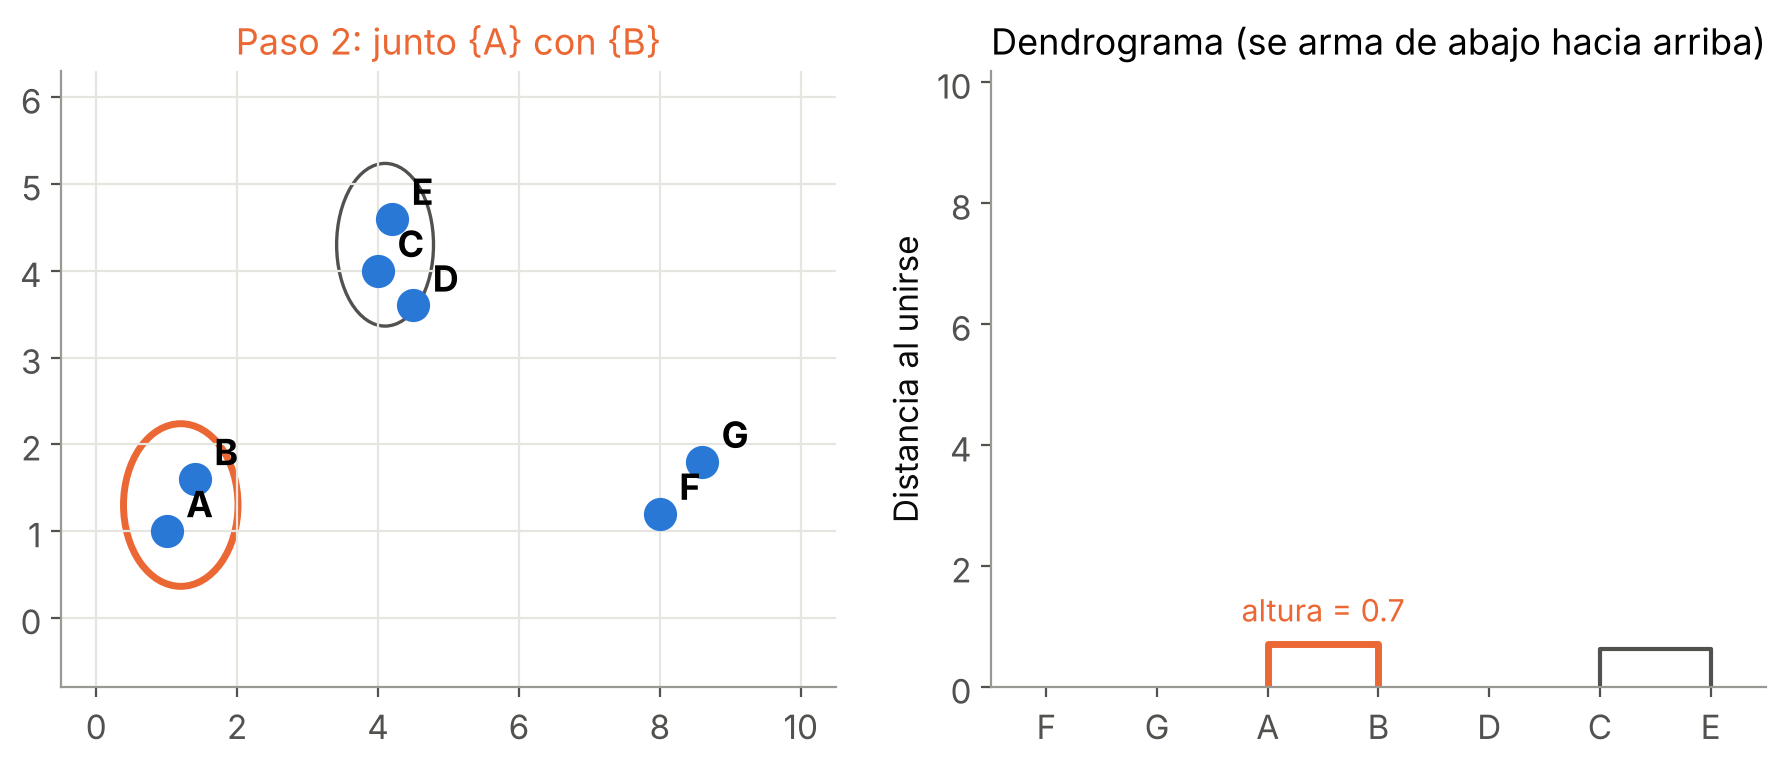
\includegraphics[width=0.88\textwidth]{img/jer_paso2.png}}%
    \only<3>{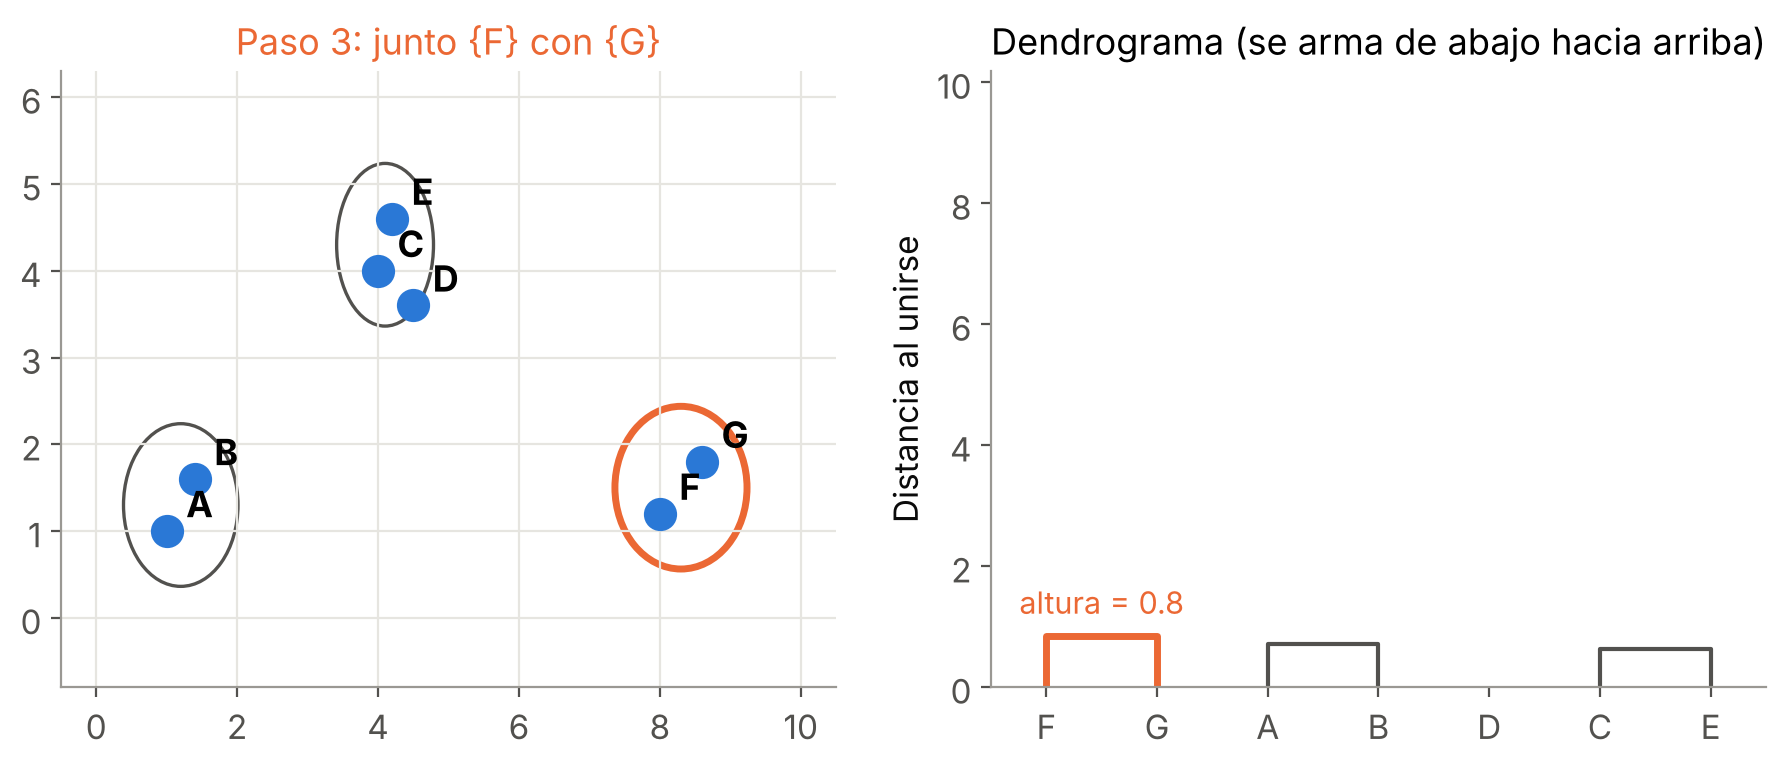
\includegraphics[width=0.88\textwidth]{img/jer_paso3.png}}%
    \only<4>{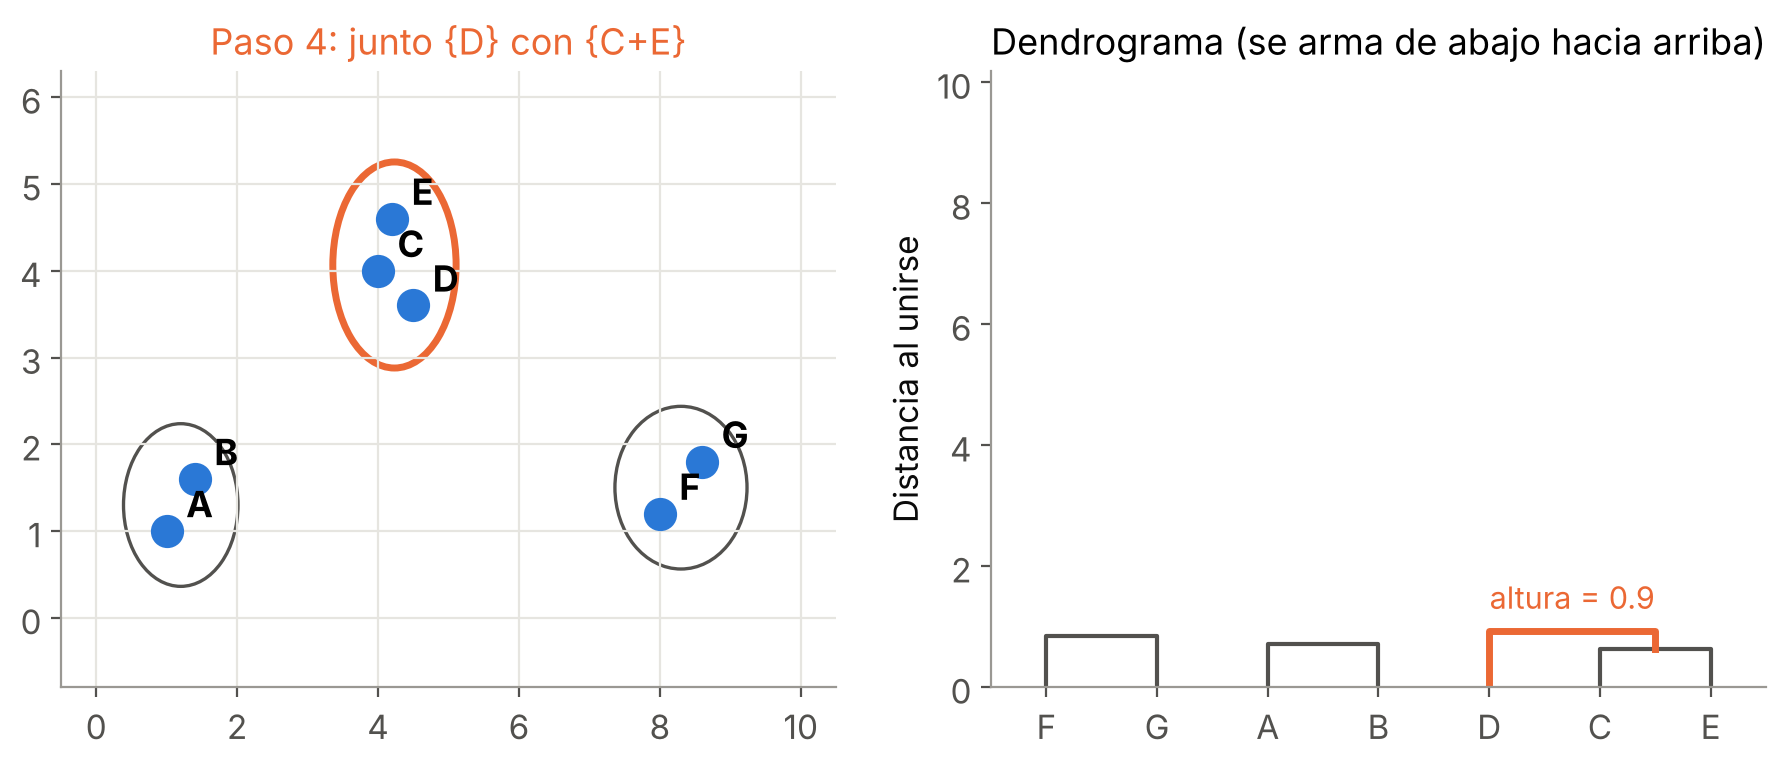
\includegraphics[width=0.88\textwidth]{img/jer_paso4.png}}%
    \only<5>{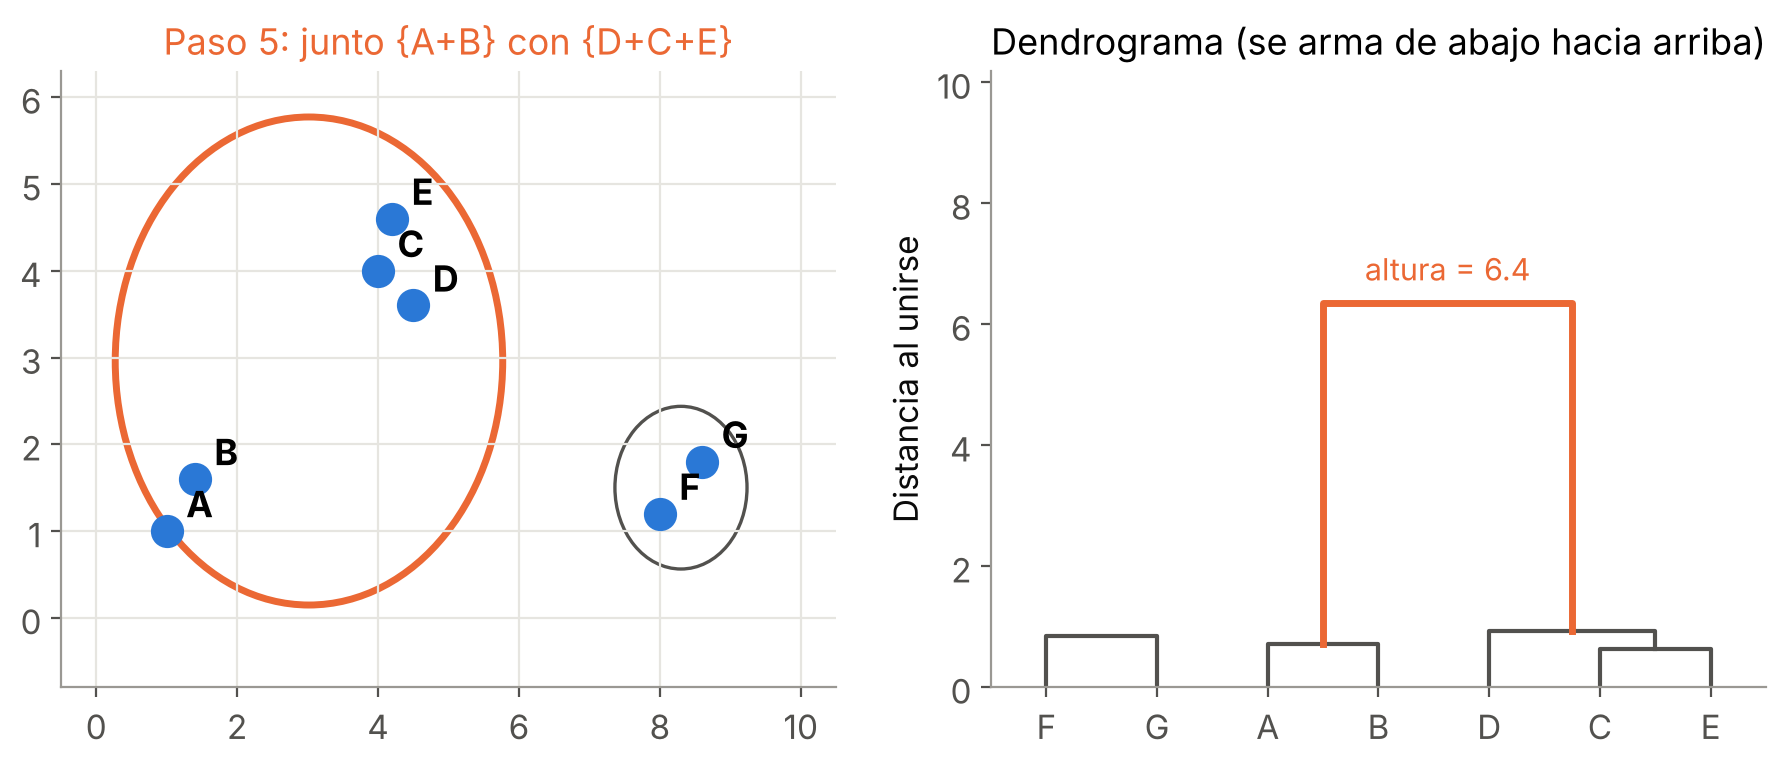
\includegraphics[width=0.88\textwidth]{img/jer_paso5.png}}%
    \only<6>{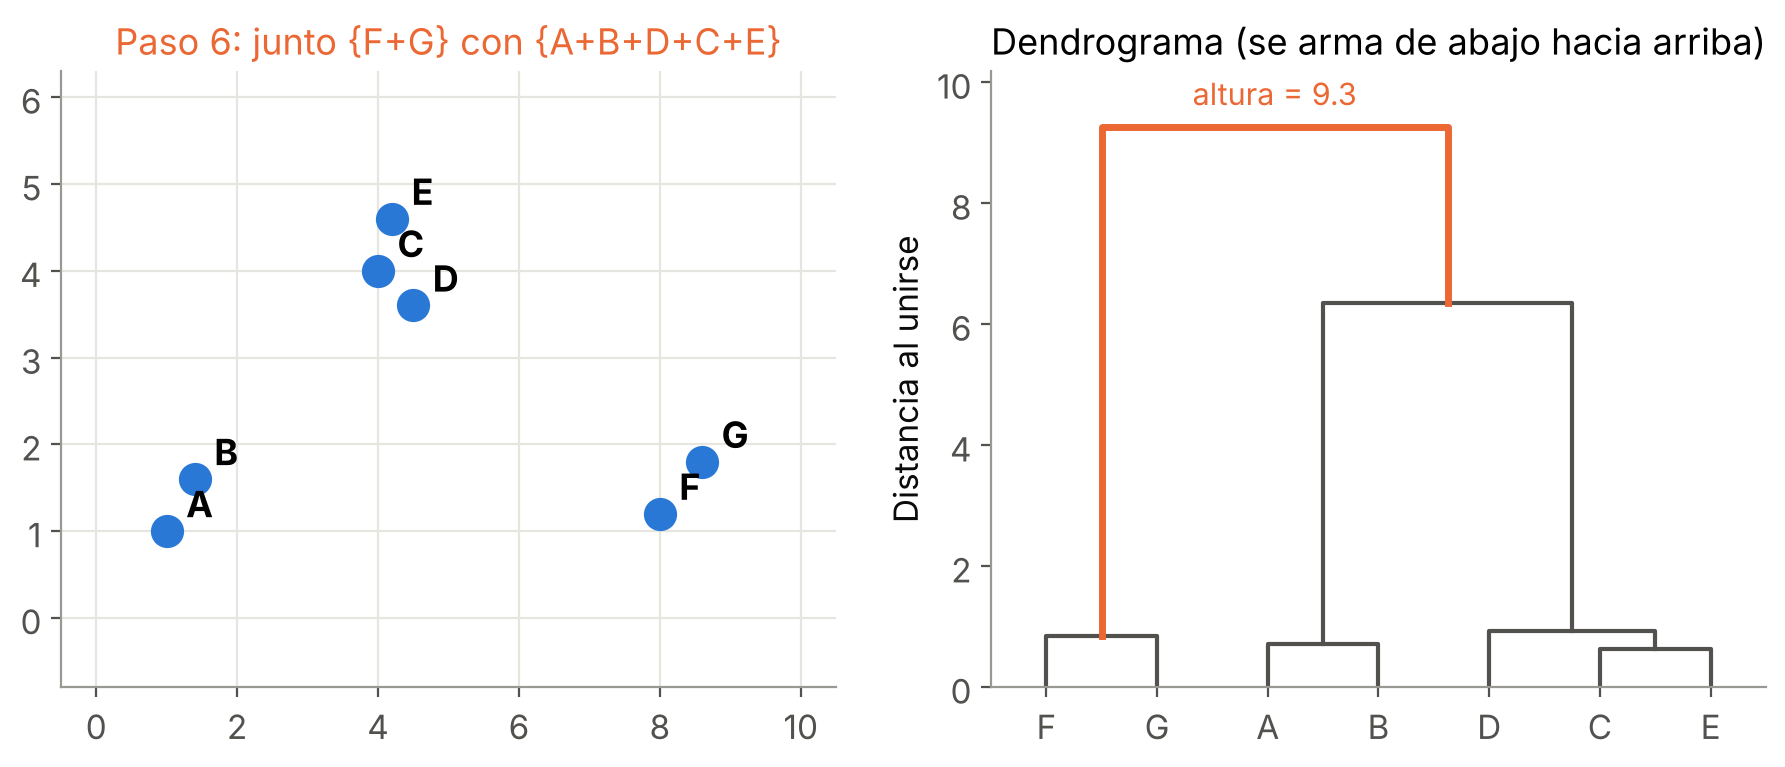
\includegraphics[width=0.88\textwidth]{img/jer_paso6.png}}%
    \par\vspace{0.4em}
    \small
    \only<1>{Los dos puntos \textbf{más cercanos} (C y E) se juntan primero. En el árbol aparece una ``U'' \textbf{bajita}: eran muy parecidos.}%
    \only<2>{Siguiente par más cercano: A y B. Otra ``U'' bajita.}%
    \only<3>{F y G. Ya tenemos 3 grupitos bien apretados.}%
    \only<4>{D se suma al grupo {C, E}. Ahora quedan 3 grupos: {A,B}, {C,D,E} y {F,G}.}%
    \only<5>{Ahora sí hay que juntar grupos \alert{lejanos}: la ``U'' sube mucho (altura 6.4). Ese \textbf{salto} es la señal de que estamos mezclando cosas distintas.}%
    \only<6>{Última unión: todo queda en un solo grupo. El árbol está completo.}%
\end{frame}

\begin{frame}{¿Cuántos grupos? Corto el árbol}
    \centering
    \only<1>{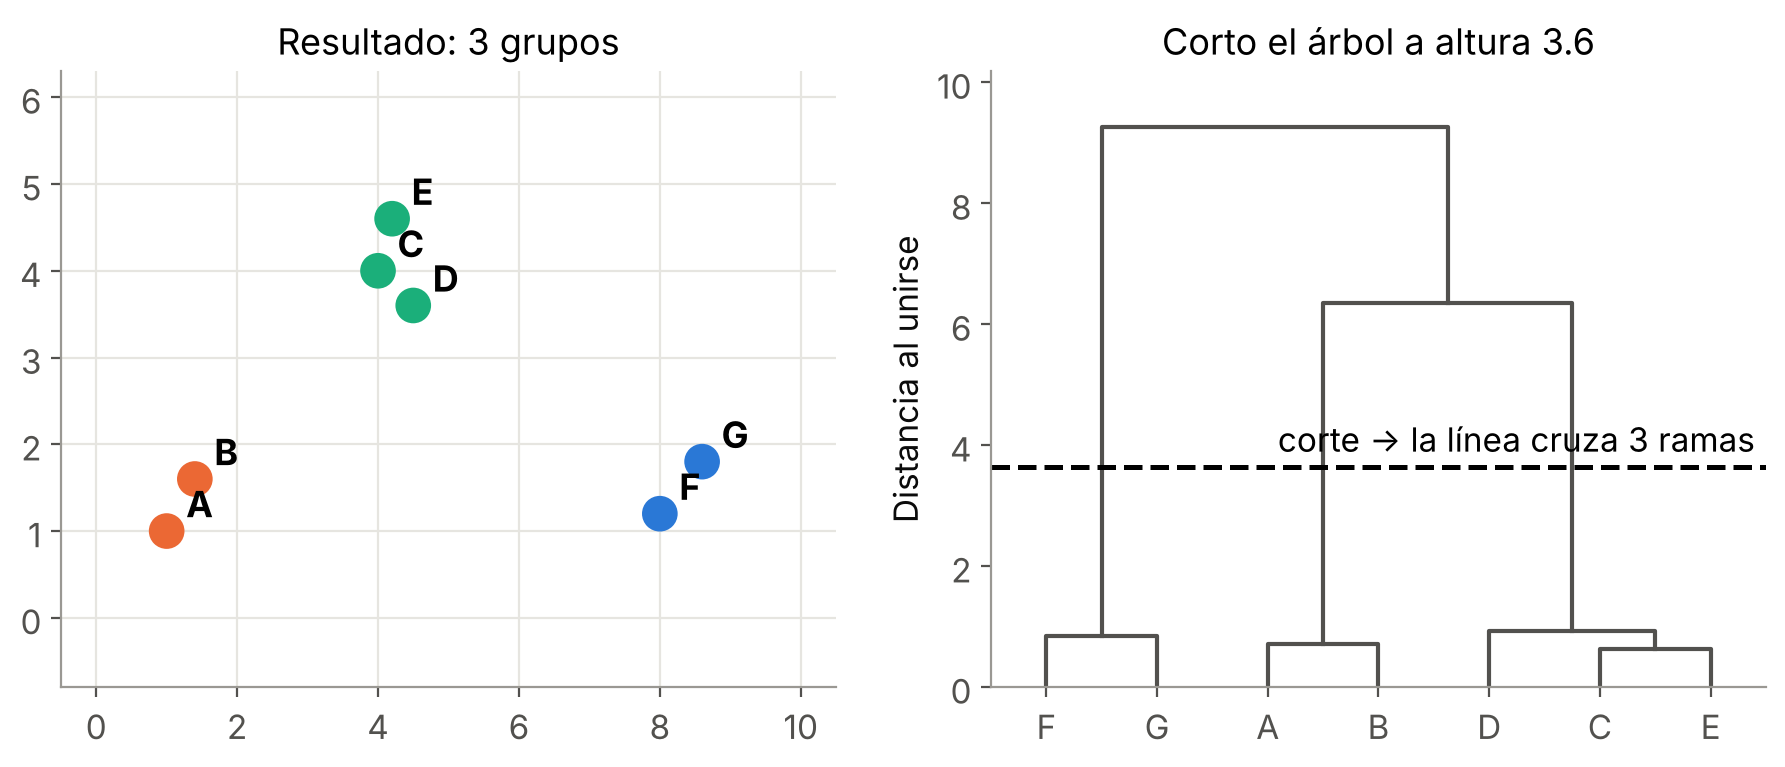
\includegraphics[width=0.88\textwidth]{img/jer_corte3.png}}%
    \only<2>{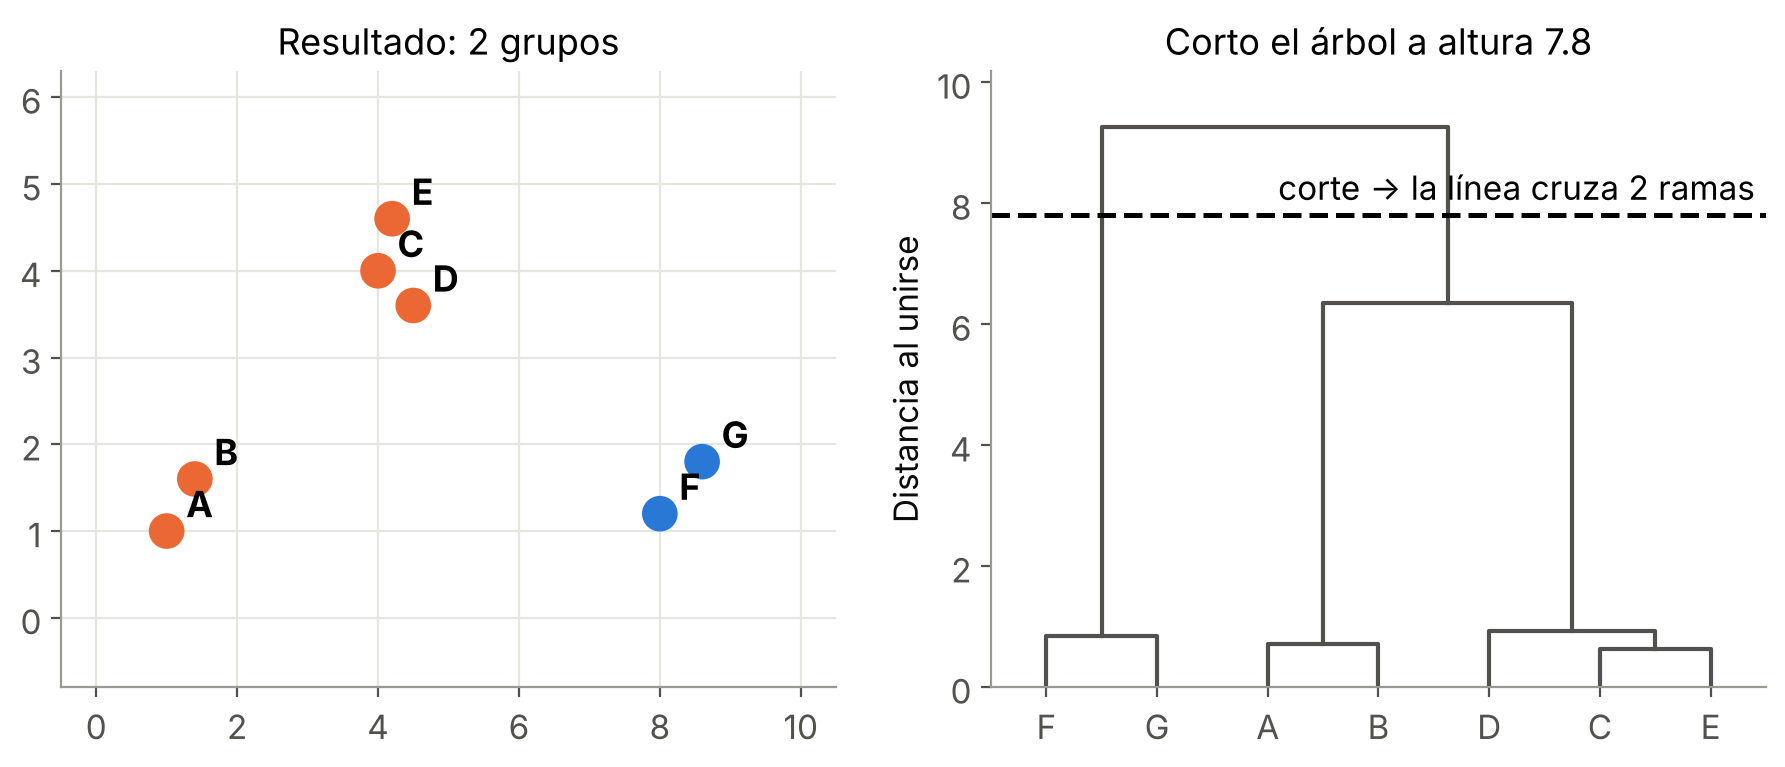
\includegraphics[width=0.88\textwidth]{img/jer_corte2.png}}%
    \par\vspace{0.4em}
    \small
    Trazo una \textbf{línea horizontal}: la cantidad de ramas que corta = la cantidad de grupos.
    \only<1>{Cortando por \textbf{debajo del gran salto} quedan 3 grupos que tienen sentido.}%
    \only<2>{Si corto más arriba, quedan 2 grupos más ``gruesos''. ¿Cuál conviene? Depende de la pregunta de negocio.}%
\end{frame}

\begin{frame}{Ahora con datos reales: países de América}
    \centering
    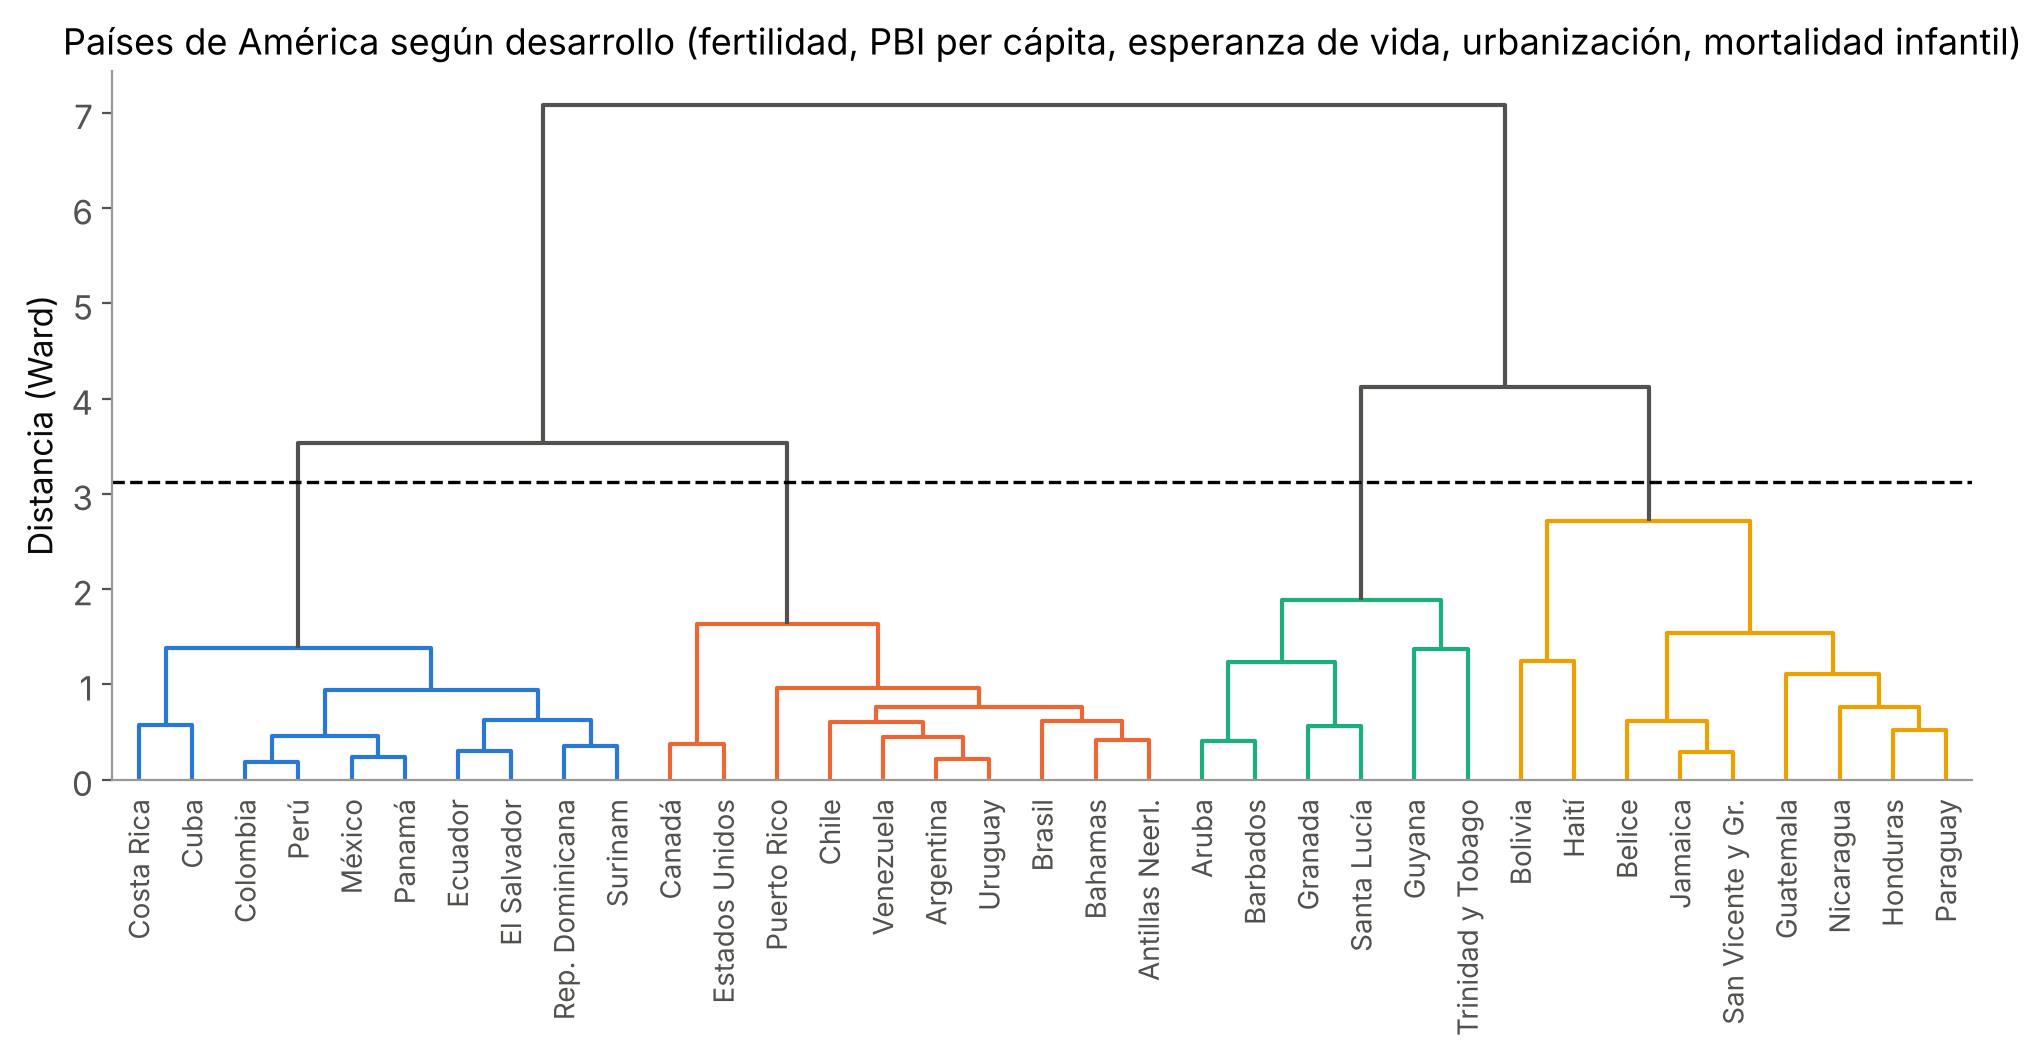
\includegraphics[height=0.6\textheight]{img/jer_america.png}\par
    \small
    \begin{itemize}
        \item Argentina y Uruguay se juntan \textbf{muy abajo}: son muy parecidos en estos indicadores.
        \item El \alert{salto grande} está alrededor de 3: si corto ahí (línea punteada) quedan 4 grupos de países.
    \end{itemize}
\end{frame}

\begin{frame}{La matemática, muy por arriba: ¿cómo mido la distancia entre grupos?}
    Entre dos países es fácil: la misma distancia en línea recta que en K-means. Pero cuando ya tengo \textbf{grupos}, hay que decidir cómo compararlos. A eso se le dice \alert{linkage}:
    \vspace{0.5em}

    \renewcommand{\arraystretch}{1.3}
    \begin{tabular}{@{}ll@{}}
        \textbf{single} & los dos miembros \textbf{más cercanos} $\rightarrow$ arma ``cadenas'', no sirve para segmentar \\
        \textbf{complete} & los dos miembros \textbf{más lejanos} \\
        \textbf{average} & el \textbf{promedio} de todas las distancias \\
        \textbf{ward} & junta los grupos que quedan \textbf{más apretados} (como K-means) \\
    \end{tabular}
    \vspace{0.8em}

    En la práctica: \textbf{usamos Ward}. En la demo se ve qué pasa con los otros.
\end{frame}

\begin{frame}{Con todos los países}
    \centering
    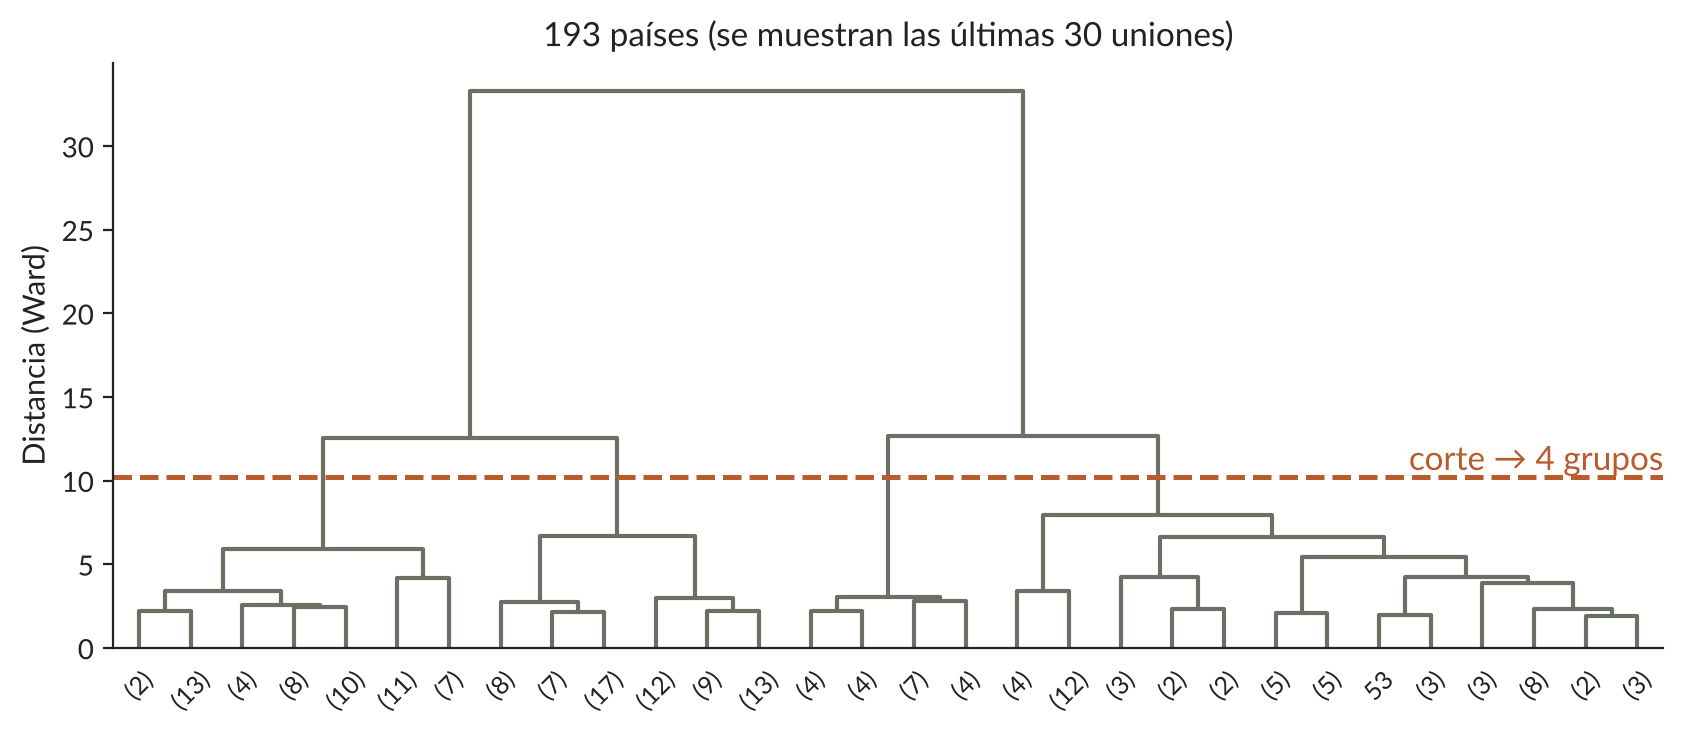
\includegraphics[width=0.75\textwidth]{img/jer_todos.png}
    \vspace{0.3em}

    \small
    \begin{tabular}{@{}lrrrr@{}}
        \toprule
        \textbf{Grupo} (mediana) & \textbf{Países} & \textbf{PBI p/c (USD)} & \textbf{Esp. vida} & \textbf{Hijos/mujer} \\
        \midrule
        Alto desarrollo (incluye Argentina) & 66 & 20.556 & 80,7 & 1,9 \\
        Desarrollo medio-alto & 55 & 4.496 & 77,3 & 2,0 \\
        Desarrollo medio-bajo & 53 & 1.240 & 64,4 & 3,8 \\
        Bajo desarrollo & 19 & 451 & 53,1 & 5,5 \\
        \bottomrule
    \end{tabular}
\end{frame}

\begin{frame}{K-means vs. jerárquico}
    \centering
    \renewcommand{\arraystretch}{1.4}
    \begin{tabular}{@{}p{3.6cm}p{4.6cm}p{4.6cm}@{}}
        \toprule
        & \textbf{K-means} & \textbf{Jerárquico} \\
        \midrule
        ¿Elijo K antes? & Sí & No: corto el árbol después \\
        Resultado & Grupos + centroides & Árbol completo (dendrograma) \\
        Cantidad de datos & Millones, sin problema & Hasta miles (es lento) \\
        Explicarlo & ``Estos son los 5 perfiles'' & ``Mirá quién se parece a quién'' \\
        ¿Mismo resultado si lo corro de nuevo? & Depende del arranque & Sí, siempre \\
        \bottomrule
    \end{tabular}
\end{frame}

\begin{frame}[standout]
    \centering
    {\Large Demo 2: ¿qué países se parecen?\par}
    \vspace{0.6em}
    {\normalsize\texttt{02\_jerarquico\_paises.ipynb}\par}
\end{frame}

% =====================================================================
\section{PCA: resumir muchas variables}

\begin{frame}{El problema}
    \begin{columns}[c]
        \column{0.45\textwidth}
        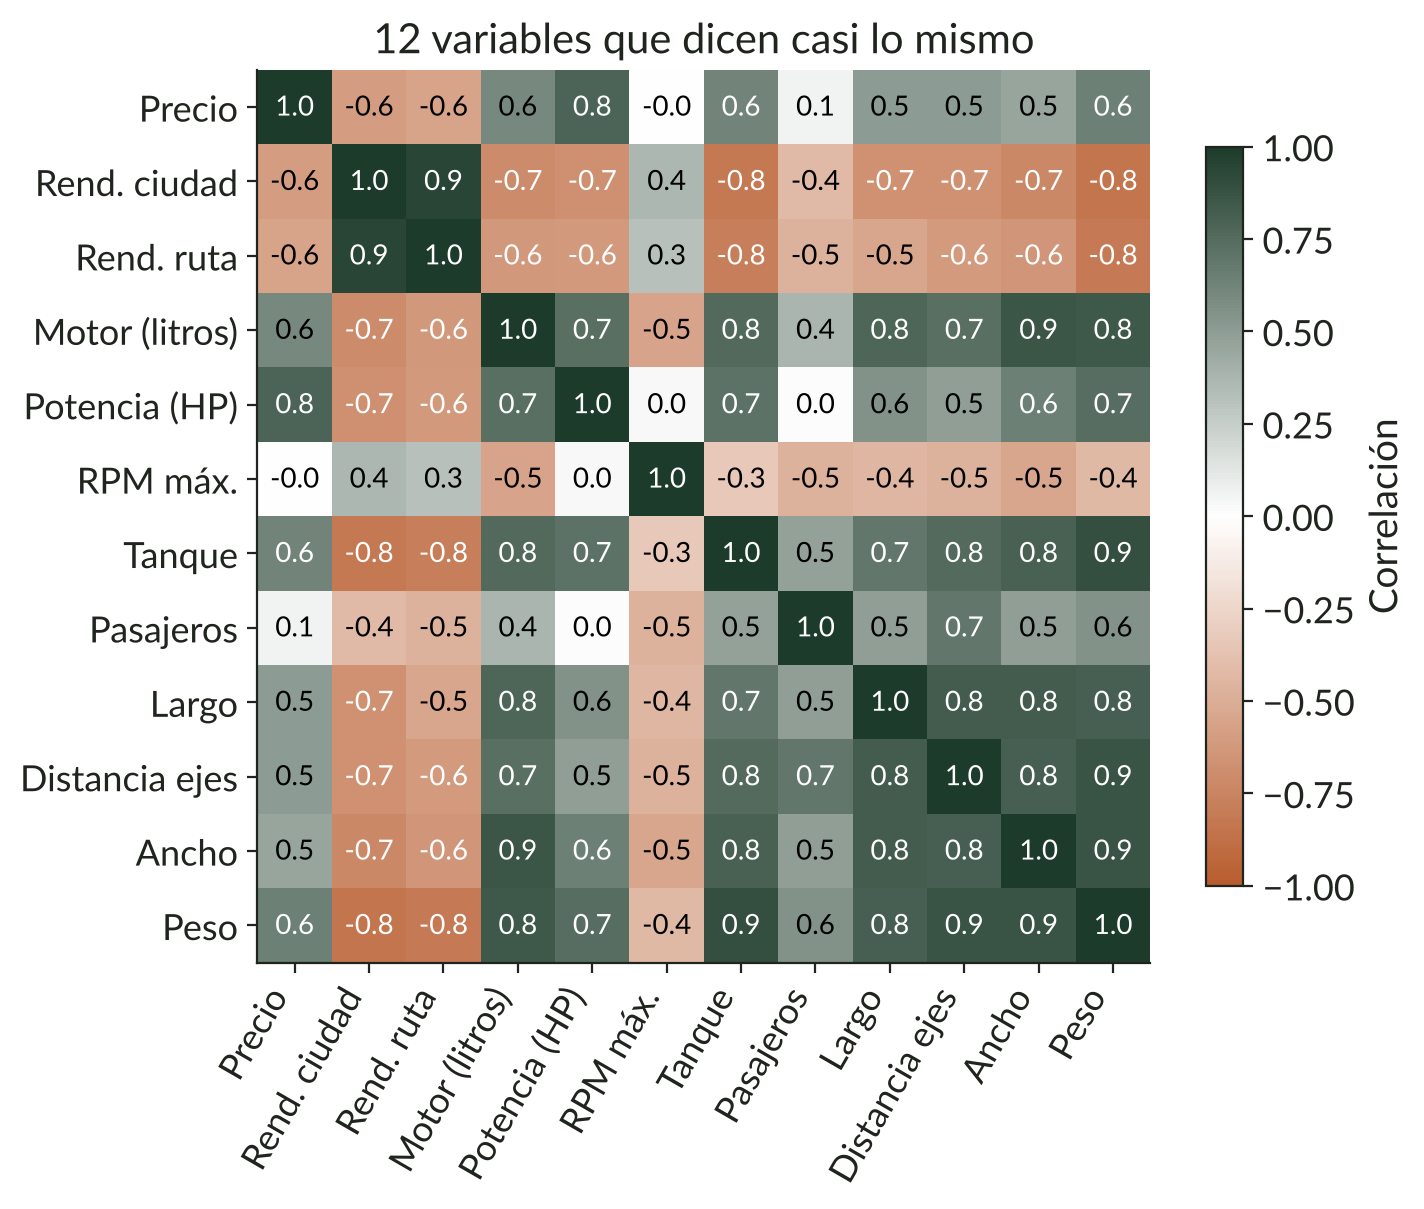
\includegraphics[width=\textwidth]{img/pca_correlaciones.png}
        \column{0.52\textwidth}
        Trabajamos en una automotriz. Queremos ver \textbf{cómo están posicionados} los 93 modelos del mercado: ¿dónde hay competencia?, ¿hay huecos?
        \vspace{0.6em}

        Tenemos 12 características por modelo, pero:
        \begin{itemize}
            \item No se pueden graficar 12 dimensiones.
            \item Muchas \alert{dicen lo mismo}: peso, largo, ancho, motor... todas miden ``qué tan grande es''.
        \end{itemize}
    \end{columns}
\end{frame}

\begin{frame}{La idea: buscar la dirección donde los datos más varían}
    \centering
    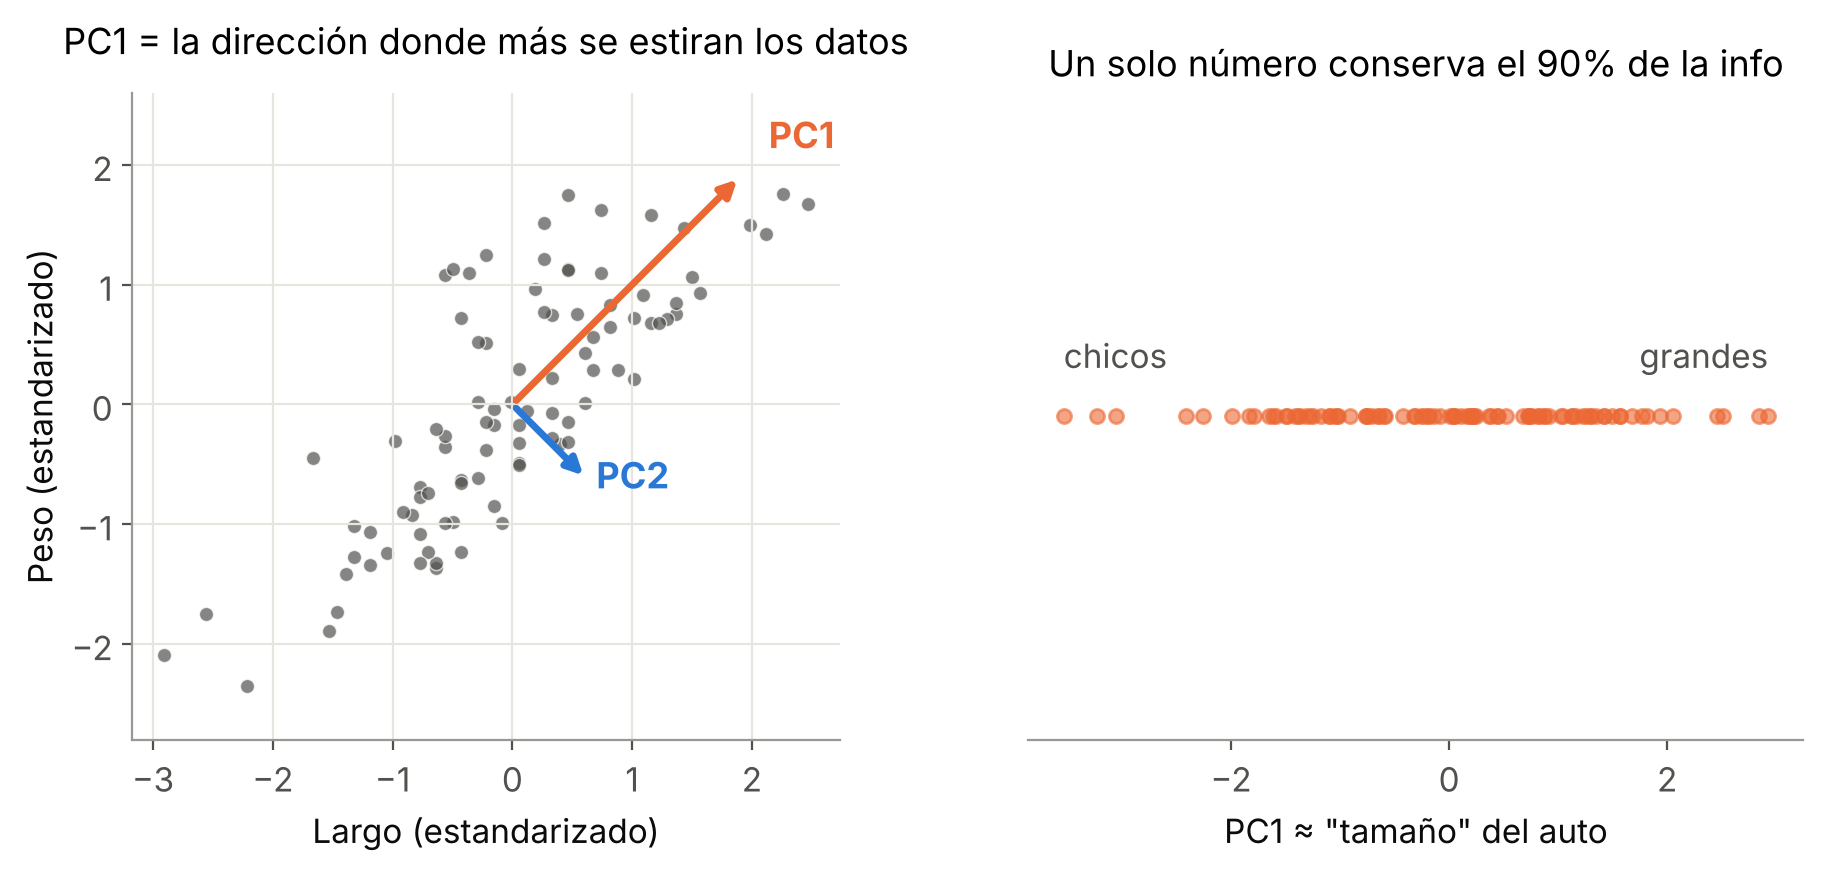
\includegraphics[width=0.8\textwidth]{img/pca_idea.png}\par
    \small
    Largo y peso van juntos. Si giro los ejes y miro solo \textbf{PC1}, con \textbf{un número} conservo casi toda la información. Ese número es, en la práctica, el ``tamaño'' del auto.
\end{frame}

\begin{frame}{La matemática, muy por arriba}
    Cada componente principal es una \alert{receta}: una suma ponderada de las variables originales (estandarizadas).
    \[
        \text{PC1} = w_1 \cdot \text{precio} + w_2 \cdot \text{rendimiento} + \dots + w_{12} \cdot \text{peso}
    \]
    \begin{itemize}
        \item PCA elige los pesos $w$ (\textbf{loadings}) para que PC1 tenga la \textbf{mayor varianza posible}.
        \item PC2 hace lo mismo con lo que sobra, \textbf{sin repetir} información de PC1 (son perpendiculares). Y así sucesivamente.
        \item Hay tantas componentes como variables, pero las primeras concentran casi todo.
        \item Igual que en clustering: \alert{estandarizar antes}, si no gana la variable con números más grandes.
    \end{itemize}
\end{frame}

\begin{frame}{¿Cuántas componentes me quedo?}
    \centering
    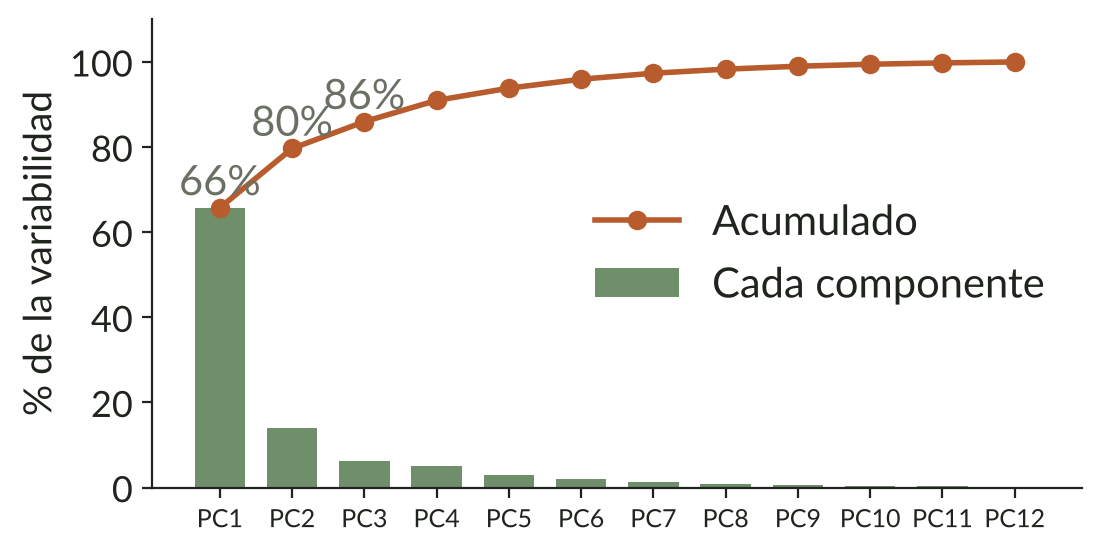
\includegraphics[width=0.62\textwidth]{img/pca_varianza.png}
    \small
    \begin{itemize}
        \item Mirar el \textbf{acumulado}: ¿con cuántas llego a 80--90\%?
        \item Para \textbf{visualizar}: 2 (o 3). Para \textbf{modelar}: las que hagan falta.
    \end{itemize}
\end{frame}

\begin{frame}{PCA no le pone nombre: lo hacemos nosotros}
    \centering
    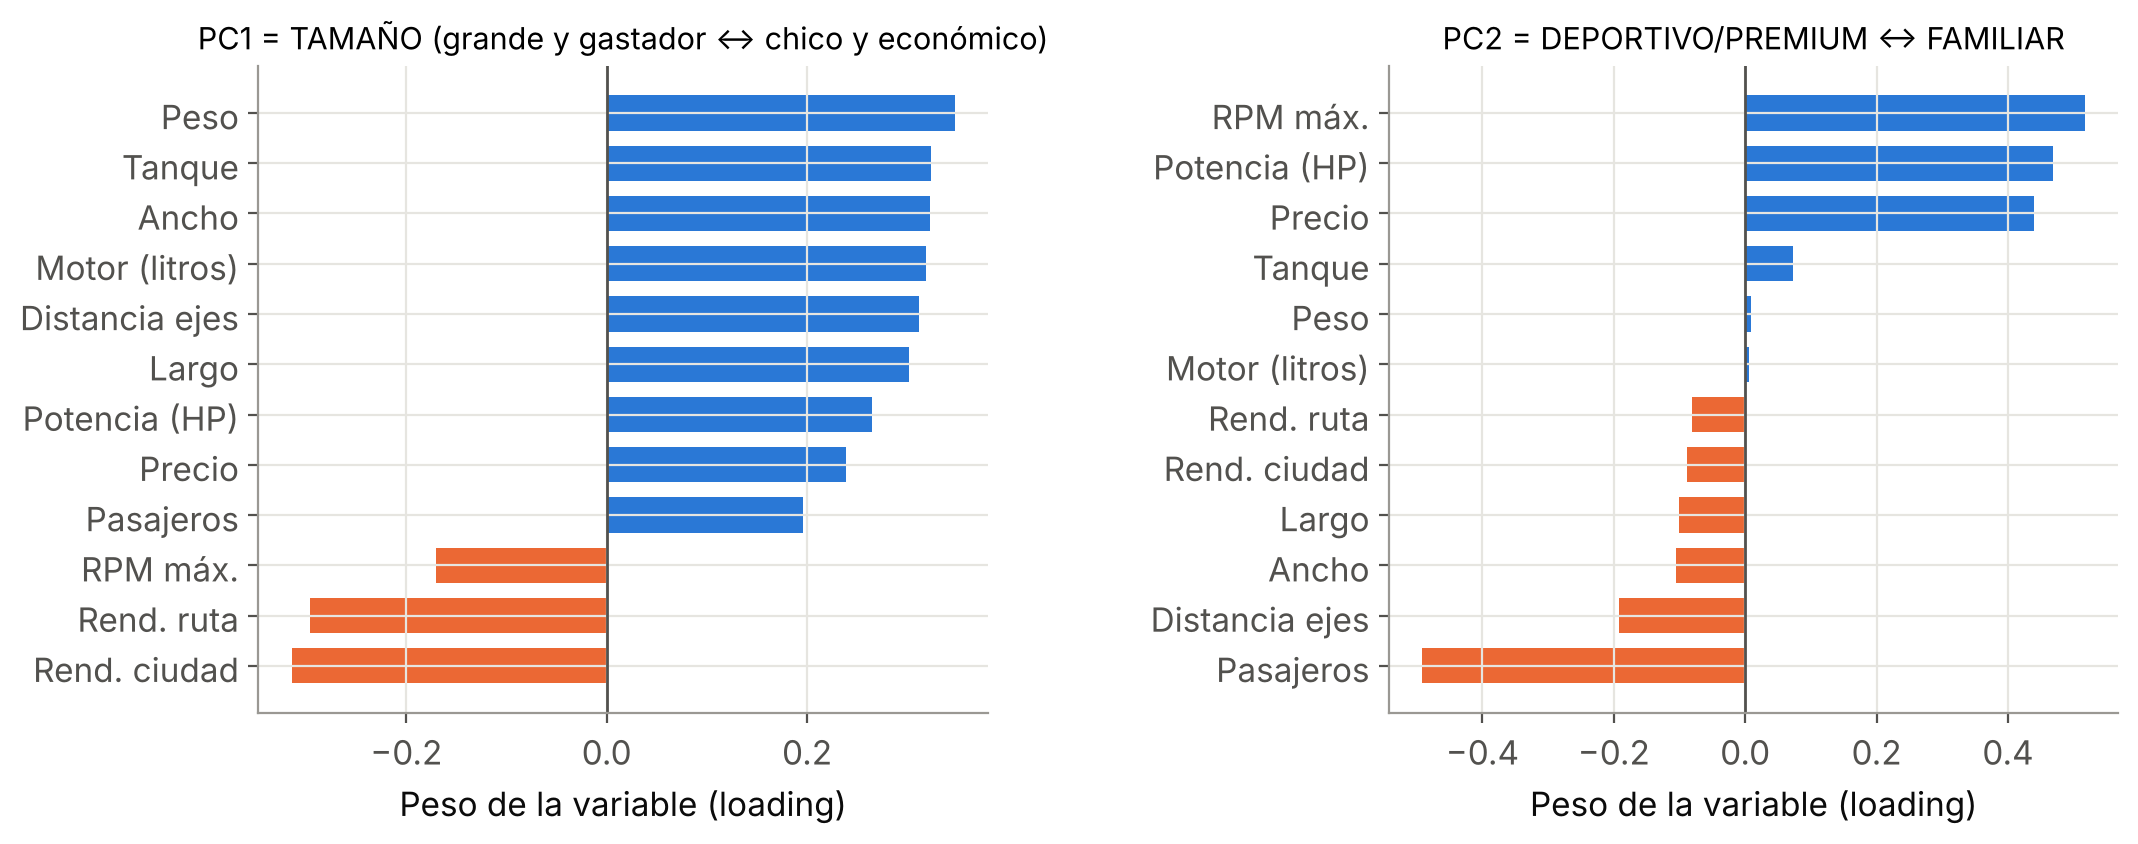
\includegraphics[width=0.92\textwidth]{img/pca_loadings.png}\par
    \small
    Mirando los loadings: \textbf{PC1 = tamaño} (todo lo ``grande'' suma, el rendimiento resta). \textbf{PC2 = deportivo/premium vs. familiar} (potencia y precio suman, pasajeros resta).
\end{frame}

\begin{frame}{El resultado: un mapa de posicionamiento}
    \begin{columns}[c]
        \column{0.62\textwidth}
        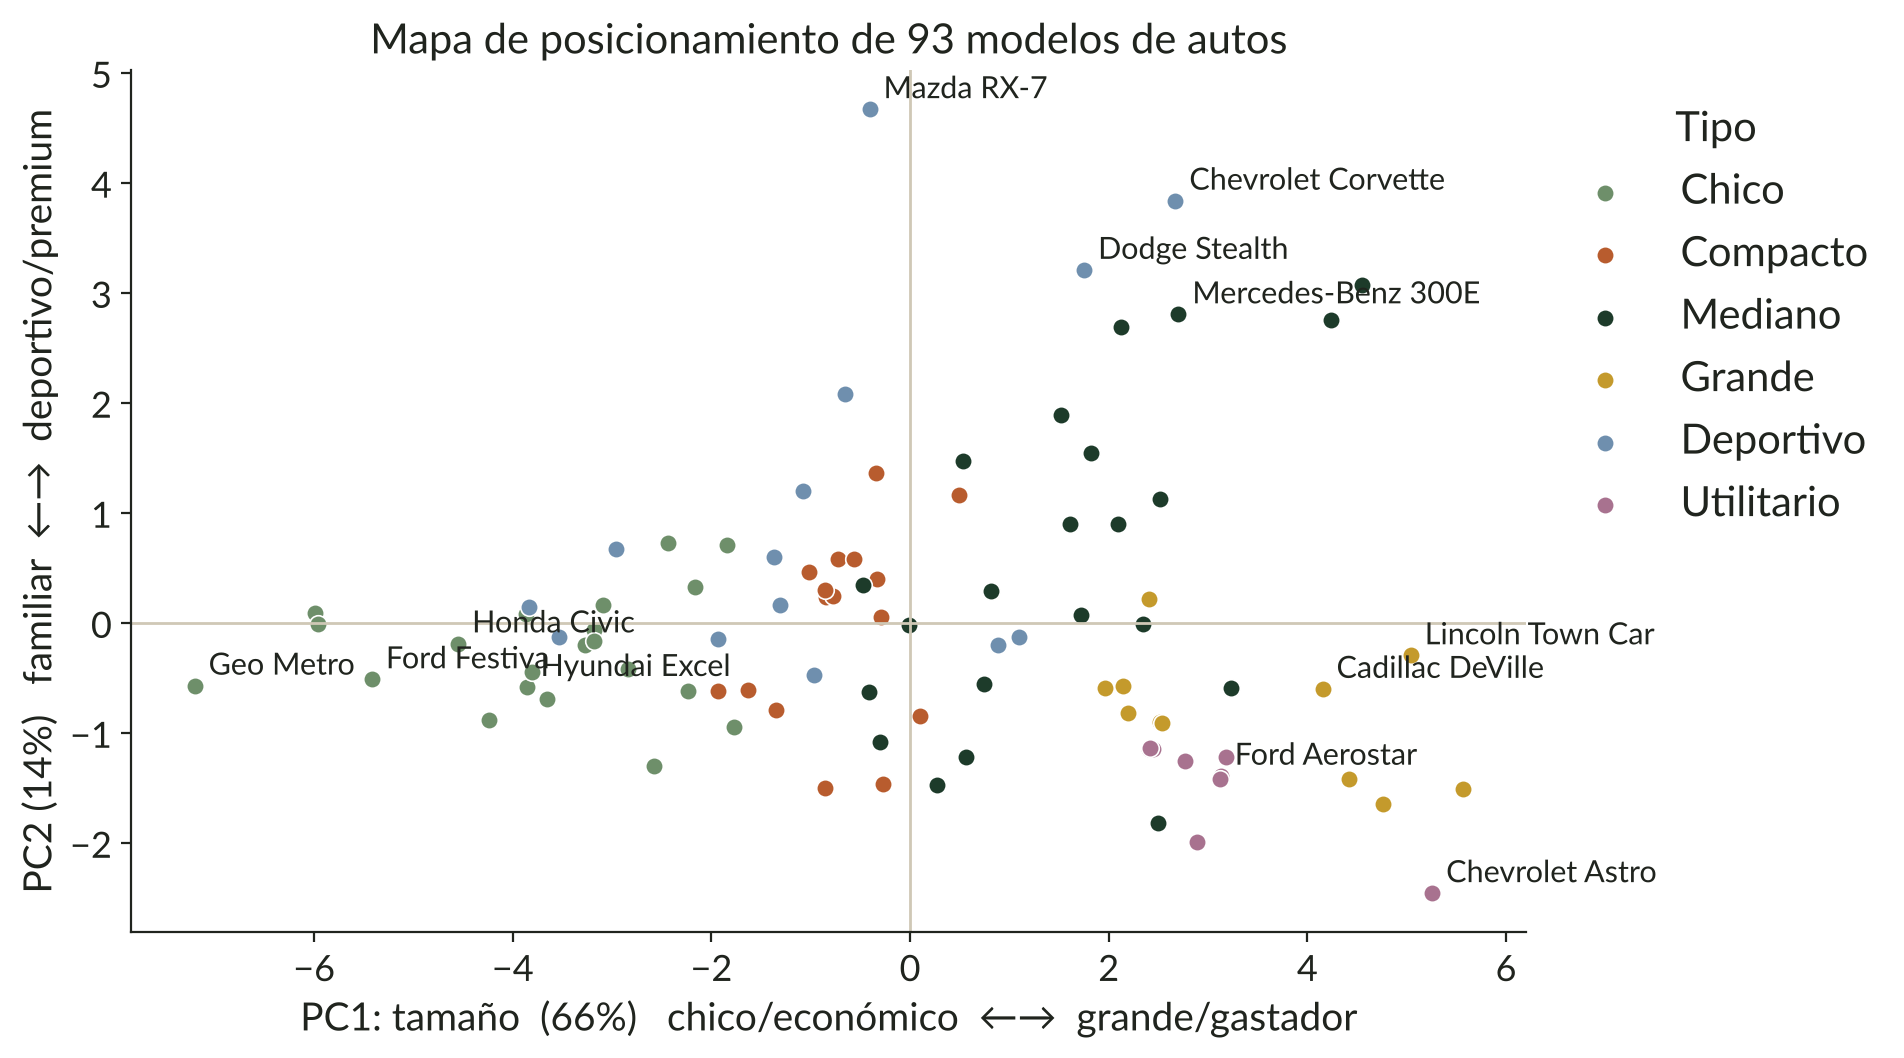
\includegraphics[width=\textwidth]{img/pca_mapa.png}
        \column{0.36\textwidth}
        \small
        \begin{itemize}
            \item El \textbf{tipo de auto no se usó}, y aun así queda ordenado: las componentes capturan algo real.
            \item Vecinos en el mapa = \textbf{competidores directos}.
            \item \alert{¿Huecos?} Grande \textit{y} deportivo: casi vacío.
        \end{itemize}
    \end{columns}
\end{frame}

\begin{frame}{Cuidado con PCA}
    \begin{itemize}
        \item \textbf{Estandarizar} antes.
        \item Las componentes son \textbf{difíciles de explicar}: ``subió PC3'' no le dice nada a nadie. En un modelo predictivo perdés explicabilidad.
        \item Solo captura relaciones \textbf{lineales}.
        \item Solo variables numéricas.
        \item Muy útil para \textbf{visualizar}, armar \textbf{índices} (ej. ``índice de desarrollo'') y como paso previo a clustering.
    \end{itemize}
\end{frame}

\begin{frame}[standout]
    \centering
    {\Large Demo 3: mapa de posicionamiento\par}
    \vspace{0.6em}
    {\normalsize\texttt{03\_pca\_autos.ipynb}\par}
\end{frame}

% =====================================================================
\begin{frame}{Resumen}
    \centering
    \renewcommand{\arraystretch}{1.4}
    \small
    \begin{tabular}{@{}p{2.5cm}p{3.6cm}p{3.6cm}p{3.6cm}@{}}
        \toprule
        & \textbf{K-means} & \textbf{Jerárquico} & \textbf{PCA} \\
        \midrule
        Hace & Agrupa filas en K grupos & Arma un árbol de parecidos & Resume columnas \\
        Usalo para & Segmentar muchos clientes & Pocos casos, sin K claro & Mapas, índices, quitar redundancia \\
        Decidís vos & K & Dónde cortar, linkage & Cuántas componentes \\
        Siempre & \multicolumn{3}{l}{Estandarizar \;·\; interpretar y ponerle nombre \;·\; validar con el negocio} \\
        \bottomrule
    \end{tabular}
    \vspace{0.8em}

    \textbf{Se combinan}: PCA para resumir $\rightarrow$ clustering sobre las componentes (bonus en la demo 3).
\end{frame}

\begin{frame}{Terminamos}
    \begin{center}
        \Large{\textbf{¿Dudas?\\¿Consultas?}}
    \end{center}
    \udesalogo{south}
\end{frame}

\end{document}
